\documentclass[12pt,letterpaper]{exam}
\usepackage[lmargin=1in,rmargin=1in,tmargin=1in,bmargin=1in]{geometry}
\usepackage{../style/exams}

% -------------------
% Course & Exam Information
% -------------------
\newcommand{\course}{MAT 101: Exam 3}
\newcommand{\term}{Fall -- 2023}
\newcommand{\examdate}{12/13/2023}
\newcommand{\timelimit}{85 Minutes}

\setbool{hideans}{true} % Student: True; Instructor: False

% -------------------
% Content
% -------------------
\begin{document}

\examtitle
\instructions{Write your name on the appropriate line on the exam cover sheet. This exam contains \numpages\ pages (including this cover page) and \numquestions\ questions. Check that you have every page of the exam. Answer the questions in the spaces provided on the question sheets. Be sure to answer every part of each question and show all your work. If you run out of room for an answer, continue on the back of the page --- being sure to indicate the problem number.} 
\scores
\bottomline
\newpage

% ---------
% Questions
% ---------
\begin{questions}

% Question 1
\newpage
\question[10] Without using a calculator and showing all your work, solve the following system of equations:
	\[
	\begin{cases}
	4x + 2y= -4 \\
	6x - 5y= 18
	\end{cases}
	\]



% Question 2
\newpage
\question[10] Consider the quadratic function $f(x)= 9 - 2(x + 5)^2$.
	\begin{enumerate}[(a)]
	\item Find the vertex of $f(x)$ and axis of symmetry. 
	\item Does $f(x)$ open upwards or downwards?
	\item Is $f(x)$ convex or concave?
	\item Does $f(x)$ have a maximum or a minimum? Find whichever value exists. 
	\item Find $a, b, c$ for the standard form for $f(x)$. 
	\end{enumerate}



% Question 3
\newpage
\question[10] Without using a calculator and showing all your work, find the vertex form for $2x^2 + 4x + 1$. 



% Question 4
\newpage
\question[10] Without using a calculator and showing all your work, factor the following polynomials as much as possible (if they cannot be factored, state so):
	\begin{enumerate}[(a)]
	\item $3x^2 + 36x - 84$
	\item $16x^4 - 1$
	\end{enumerate}



% Question 5
\newpage
\question[10] Without using a calculator and showing all your work, factor the polynomial $6x^2 - 11x - 7$ as much as possible. If it cannot be factored, state so and explain why. 



% Question 6
\newpage
\question[10] Find the equation of the quadratic function plotted below. 
	\[
	\fbox{
	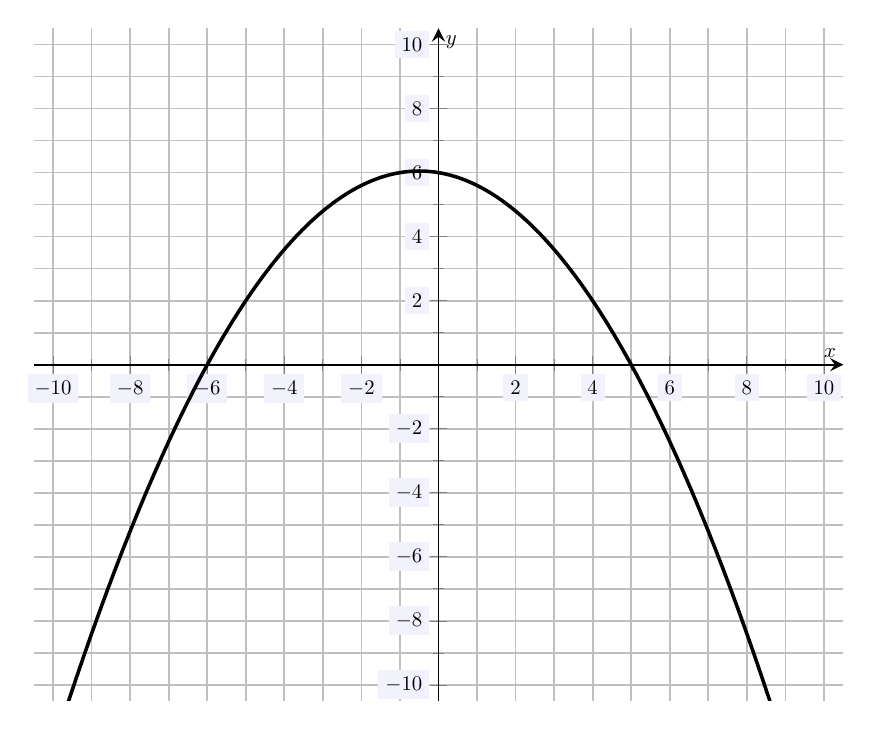
\begin{tikzpicture}[scale=1.5,every node/.style={scale=0.5}]
	\begin{axis}[
	grid=both,
	axis lines=middle,
	ticklabel style={fill=blue!5!white},
	xmin= -10.5, xmax=10.5,
	ymin= -10.5, ymax=10.5,
	xtick={-10,-8,-6,-4,-2,0,2,4,6,8,10},
	ytick={-10,-8,-6,-4,-2,0,2,4,6,8,10},
	minor tick = {-10,-9,...,10},
	xlabel=\(x\),ylabel=\(y\),
	]
	\addplot[line width=0.03cm,domain=-10:10,samples=100] ({x},{1/5*(-x^2 - x + 30)});
	\end{axis}
	\end{tikzpicture}
	}
	\]



% Question 7
\newpage
\question[10] Without using a calculator and showing all your work, find the exact solution(s) to the following equation:
	\[
	x(x + 3)= 18
	\]



% Question 8
\newpage
\question[10] Without using a calculator and showing all your work, find the exact solution(s) to the following equation by using the quadratic formula:
	\[
	\dfrac{5x - 1}{x}= \dfrac{6x}{x - 1}
	\]



% Question 9
\newpage
\question[10] Consider the polynomial $p(x)= 9x^3 (x + 1) (x - 3)^2 (x + 6)^4 (x - 7)^9$.
	\begin{enumerate}[(a)]
	\item Find the degree of $p(x)$. 
	\item How many \textit{distinct} roots does $p(x)$ have?
	\item Find the roots of $p(x)$ along with their multiplicities. 
	\item Do the `ends' of $p(x)$ `point' in the same direction or opposite? Explain. 
	\item Does $p(x)$ have a maximum, minimum, both, or neither?
	\end{enumerate} 



% Question 10
\newpage
\question[10] Find the equation of the polynomial $p(x)$ plotted below, if $\deg p(x)= 6$. 
	\[
	\fbox{
	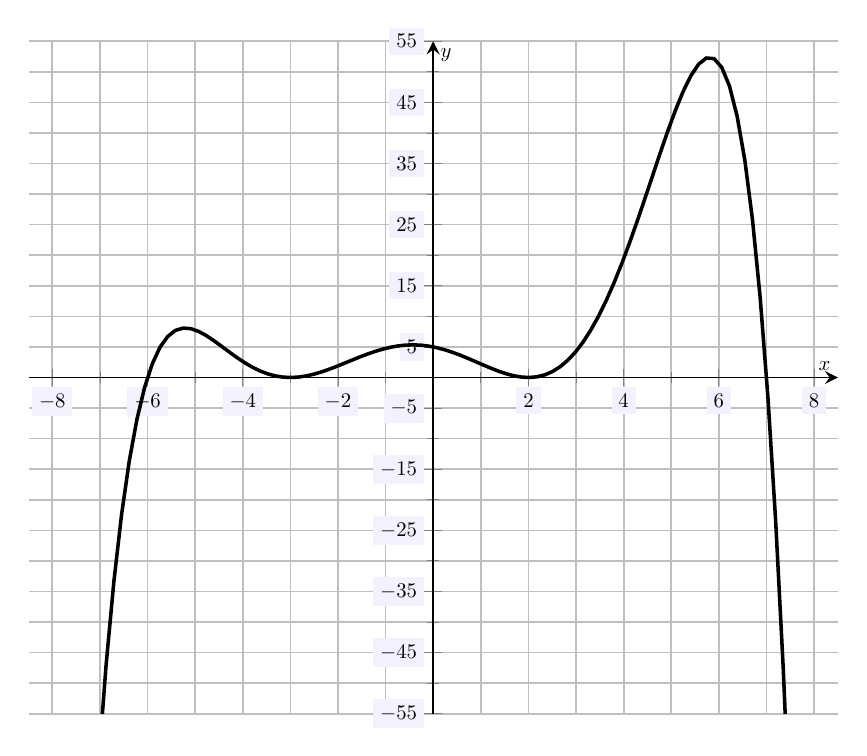
\begin{tikzpicture}[scale=1.5,every node/.style={scale=0.5}]
	\begin{axis}[
	grid=both,
	axis lines=middle,
	ticklabel style={fill=blue!5!white},
	xmin= -8.5, xmax=8.5,
	ymin= -55, ymax=55,
	xtick={-10,-8,-6,-4,-2,0,2,4,6,8,10},
	ytick={-55,-45,...,55},
%	minor tick = {-50,-40,...,50},
	minor x tick num = 1,
	minor y tick num = 1,
	xlabel=\(x\),ylabel=\(y\),
	]
	\addplot[line width=0.03cm,domain=-8:8,samples=100] ({x},{-5/1512*(x + 6)*(x + 3)^2*(x - 2)^2*(x - 7)});
	\end{axis}
	\end{tikzpicture}
	}
	\]	


\end{questions}
\end{document}